
%----------------------------------------------------------------------------
\chapter{Preliminaries}
%----------------------------------------------------------------------------



\section{Modeling with graphs}

Structural or behavioral modeling of systems are often done using graphs. .... \TODO{...}

\section{Runtime modeling}

In this thesis we use structural modeling to model the current state of the system. This model is called the live model, which captures the state and the operating context of the system.

\subsection{Runtime modeling example}



\section{Graph pattern matching concepts}

\begin{figure}[h]
	\begin{center}
		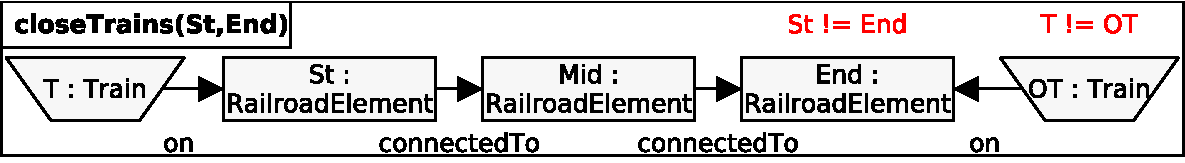
\includegraphics[width=0.75\textwidth]{figures/pattern-visual.pdf}
		\caption{Visual representation of a graph pattern}
		\label{pattern-visual}
	\end{center}
\end{figure}

A graph pattern's purpose is to define a set of constraints that can be satisfied by the vertices of the graph.

\section{Local search}

Local search is an algorithm to provide matchings of a graph pattern in a graph.

\subsection{Distributed local search}

As models are stored on different computational units we still needs to find matches, that can span over multiple model parts. To find matches for a pattern local search algorithm is used in a distributed way. Search operations are being executed locally, and if the next operation needs to be executed on multiple nodes, the search context, (ie.\ the bound variables and the operations number) are sent to other computational units.